% ========================================
% SEZIONE 1: Simmetria
% ========================================
\begin{question}[ID=1.1, subtitle={Simmetria centrale rispetto a $P(1,1)$}, tags={trasformazioni, simmetria}, difficulty=facile]
Dopo aver descritto le leggi di trasformazione di una simmetria centrale rispetto al punto $P(1,1)$.
\begin{enumerate}
\item Determinare il punto $A'$ simmetrico rispetto ad $A(5,3)$;
\item Determinare l'equazione della curva $\gamma'$ simmetrica di $\gamma: \ y+(x-2)^2 + 3 = 0 $ rispetto al punto $P$;
\item Verificare che la curva di equazione $x^2+4y^2-2x-8y+1=0$ ha centro di simmetria nel punto $P$.
\end{enumerate}
\begin{solution}
La simmetria centrale rispetto a $P(1,1)$ ha equazioni $x'=2-x,\ y'=2-y$ (il punto medio di ciascuna coppia punto–immagine è $P$).
\begin{enumerate}
\item $A(5,3)\Rightarrow A'(2-5,\ 2-3)=(-3,-1)$.
\item Si sostituisce $x\to2-x$, $y\to2-y$ nell'equazione di $\gamma$: $(2-y)+((2-x)-2)^2+3=0\Rightarrow x^2-y+5=0$, cioè $\gamma':\ y=x^2+5$ (la parabola, prima rivolta verso il basso con vertice $(2,-3)$, diventa rivolta verso l'alto con vertice $(0,5)$).
\item Completando i quadrati: $x^2-2x+4y^2-8y+1=(x-1)^2+4(y-1)^2-4=0$, cioè $(x-1)^2+4(y-1)^2=4$: ellisse di centro $(1,1)=P$. Avendo centro in $P$, è simmetrica rispetto a $P$.
\end{enumerate}
\end{solution}
\end{question}

%---------------------------------------------------------------------------------%

\begin{question}[ID=1.2, subtitle={Simmetria assiale rispetto alla retta $x=1$}, tags={trasformazioni, simmetria}, difficulty=facile]
Dopo aver descritto le leggi di trasformazione di una simmetria assiale rispetto alla retta $x=1$.
\begin{enumerate}
\item Determinare il punto $A'$ simmetrico rispetto ad $A(5,3)$;
\item Determinare l'equazione della curva $\gamma'$ simmetrica di $\gamma: \ y+(x-2)^2 + 3 = 0$;
\item Verificare che la curva di equazione $y=x^2-2x+3$ è simmetrica rispetto alla retta $x=1$
\end{enumerate}
\begin{solution}
La simmetria assiale rispetto a $x=1$ ha equazioni $x'=2-x,\ y'=y$ (cambia solo l'ascissa, riflessa attorno a $x=1$).
\begin{enumerate}
\item $A(5,3)\Rightarrow A'(2-5,\ 3)=(-3,3)$.
\item Sostituendo $x\to2-x$, $y\to y$ in $\gamma$: $y+((2-x)-2)^2+3=0\Rightarrow y+x^2+3=0$, cioè $\gamma':\ y=-x^2-3$ (vertice da $(2,-3)$ a $(0,-3)$).
\item $y=x^2-2x+3=(x-1)^2+2$: parabola di vertice $(1,2)$ e asse $x=1$. L'asse di simmetria coincide con la retta data, quindi la curva è simmetrica rispetto a $x=1$.
\end{enumerate}
\end{solution}
\end{question}


% ========================================
% SEZIONE 2: Traslazioni
% ========================================


% ========================================
% SEZIONE 3: Dilatazioni e omotetie
% ========================================
\begin{question}[ID=3.1, subtitle={Omotetia con centro $P(2,1)$ e rapporto $k=2$ sul triangolo $ABC$}, tags={trasformazioni geometriche, omotetia}, difficulty=media]
Dato il triangolo di vertici $A(0,0), \quad B(2,0), \quad C(2,2)$, determinare il corrispondente triangolo $A'B'C'$ del triangolo $ABC$ nell'omotetia avente rapporto di omotetia $k=2$ e centro $P(2,1)$.
\begin{enumerate}
\item Determinare le equazioni della trasformazione;
\item Rappresentare i due triangoli;
\item Calcolare le aree dei due triangoli.
\end{enumerate}
\begin{solution}
\begin{enumerate}
\item Omotetia di centro $P(2,1)$ e rapporto $k=2$: $x'=k(x-2)+2=2x-2$, $y'=k(y-1)+1=2y-1$.
\item Immagini dei vertici: $A(0,0)\to A'(-2,-1)$, $B(2,0)\to B'(2,-1)$, $C(2,2)\to C'(2,3)$. Si rappresentano $ABC$ (triangolo rettangolo in $B$) e $A'B'C'$ (rettangolo in $B'$), allineati lungo le rette per il centro $P$.
\item $ABC$: cateti $AB=2$ e $BC=2$, area $=\tfrac12\cdot2\cdot2=2$. $A'B'C'$: cateti $A'B'=4$ e $B'C'=4$, area $=\tfrac12\cdot4\cdot4=8$. Il rapporto delle aree è $k^2=4$, coerente con l'omotetia.
\end{enumerate}
\end{solution}
\end{question}

%---------------------------------------------------------------------------------%

\begin{question}[ID=3.2, subtitle={Dilatazione con centro nell'origine sul triangolo $ABC$}, tags={trasformazioni geometriche, dilatazione}, difficulty=media]
Dato il triangolo di vertici $A(0,0), \quad B(2,0), \quad C(2,2)$, determinare il corrispondente triangolo $A'B'C'$ del triangolo $ABC$ nella dilatazione con centro nell'origine avente equazioni di trasformazione:
\[
\begin{cases}
x' = -2x \\
y' = 3y
\end{cases}
\]
\begin{enumerate}
\item Rappresentare i due triangoli;
\item Calcolare le aree dei due triangoli.
\end{enumerate}
\begin{solution}
\begin{enumerate}
\item Immagini dei vertici con $x'=-2x,\ y'=3y$: $A(0,0)\to A'(0,0)$, $B(2,0)\to B'(-4,0)$, $C(2,2)\to C'(-4,6)$. La dilatazione raddoppia (con riflessione) le ascisse e triplica le ordinate: $A'B'C'$ è rettangolo in $B'$.
\item $ABC$: area $=\tfrac12\cdot2\cdot2=2$. $A'B'C'$: cateti $A'B'=4$ e $B'C'=6$, area $=\tfrac12\cdot4\cdot6=12$. Il rapporto è $|{-2}\cdot3|=6$, cioè il valore assoluto del prodotto dei due fattori di scala.
\end{enumerate}
\end{solution}
\end{question}

% ========================================
% SEZIONE 4: Miscellanea
% ========================================
\begin{question}[ID=4.1, subtitle={Trasformazioni della retta $y=2x+1$}, tags={trasformazioni geometriche, retta}, difficulty=media]
Data la retta $r:\; y = 2x + 1$, determina l'equazione della retta corrispondente di $r$ nei seguenti casi:
\begin{enumerate}
\item nella simmetria rispetto all'asse $x$;
\item nella traslazione che trasforma $A(1,-3)$ in $A'(4,-2)$;
\item nell'omotetia avente centro nell'origine e rapporto 3.
\end{enumerate}
\begin{solution}
\begin{enumerate}
\item Simmetria rispetto all'asse $x$: $y\to-y$, quindi $-y=2x+1\Rightarrow y=-2x-1$.
\item La traslazione ha vettore $A\to A'=(4-1,\,-2-(-3))=(3,1)$, cioè $x'=x+3,\ y'=y+1$. Sostituendo $x=x'-3,\ y=y'-1$: $y'-1=2(x'-3)+1\Rightarrow y'=2x'-4$, cioè $y=2x-4$.
\item Omotetia di centro $O$ e rapporto 3: $x'=3x,\ y'=3y$. Sostituendo $x=\tfrac{x'}{3},\ y=\tfrac{y'}{3}$: $\tfrac{y'}{3}=2\cdot\tfrac{x'}{3}+1\Rightarrow y'=2x'+3$, cioè $y=2x+3$.
\end{enumerate}
\end{solution}
\end{question}

%---------------------------------------------------------------------------------%

\begin{question}[ID=4.2, subtitle={Trasformazioni della parabola $y=x^2+2$}, tags={trasformazioni geometriche, parabola}, difficulty=media]
Data la parabola $\gamma:\; y = x^2 + 2$, determina l'equazione della curva corrispondente $\gamma'$ nei seguenti casi:
\begin{enumerate}
\item nella simmetria rispetto alla bisettrice del primo e terzo quadrante;
\item nella traslazione che trasforma $A(1,-3)$ in $A'(4,-2)$;
\item nell'omotetia avente centro nell'origine e rapporto 2.
\end{enumerate}
\begin{solution}
\begin{enumerate}
\item Simmetria rispetto a $y=x$: si scambiano $x$ e $y$, quindi $x=y^2+2$ (parabola con asse orizzontale, vertice $(2,0)$, rivolta verso destra).
\item Traslazione di vettore $(3,1)$: $x=x'-3,\ y=y'-1$, da cui $y'-1=(x'-3)^2+2\Rightarrow y'=(x'-3)^2+3$, cioè $y=x^2-6x+12$.
\item Omotetia di centro $O$ e rapporto 2: $x=\tfrac{x'}{2},\ y=\tfrac{y'}{2}$, da cui $\tfrac{y'}{2}=\big(\tfrac{x'}{2}\big)^2+2\Rightarrow y'=\tfrac{x'^2}{2}+4$, cioè $y=\tfrac{x^2}{2}+4$.
\end{enumerate}
\end{solution}
\end{question}

% ========================================
% SEZIONE 5: Grafici e valori assoluti
% ========================================
\begin{question}[ID=5.1, subtitle={Trasformazioni del grafico di $y=|x|$}, tags={trasformazioni geometriche, valore assoluto}, difficulty=media]
Applicando opportune trasformazioni geometriche al grafico della funzione $y=|x|$ deduci l'equazione delle
funzioni il cui grafico non è etichettato.
\newline

\centering
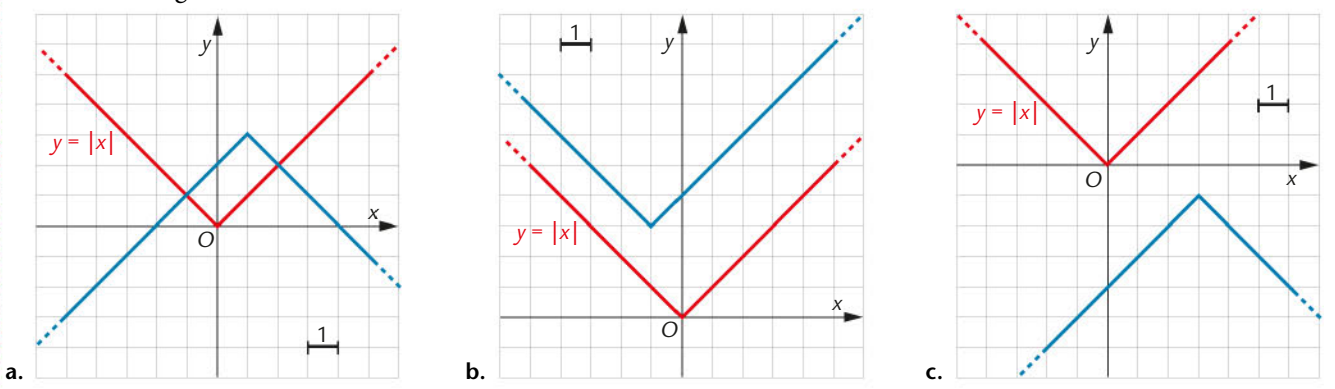
\includegraphics[width=\linewidth]{images/trasformazioni_valore_assoluto.png}
\begin{solution}
Si parte da $y=|x|$ (V con vertice nell'origine e pendenze $\pm1$) e si riconoscono le trasformazioni elementari:
\begin{itemize}
\item $y=|x-a|$: traslazione orizzontale di $a$ (vertice in $(a,0)$);
\item $y=|x|+b$: traslazione verticale di $b$ (vertice in $(0,b)$);
\item $y=-|x|$: simmetria rispetto all'asse $x$ (V capovolta);
\item $y=k|x|$: dilatazione verticale di fattore $k$ (rami più o meno ripidi).
\end{itemize}
Per ogni grafico non etichettato si individua la posizione del vertice $(a,b)$ e l'orientamento/pendenza dei rami, scrivendo quindi l'equazione nella forma $y=\pm k\,|x-a|+b$.
\end{solution}
\end{question}

%---------------------------------------------------------------------------------%

\begin{question}[ID=5.2, subtitle={Traslazione del grafico di $y=f(x)$}, tags={trasformazioni geometriche, valore assoluto}, difficulty=media]
\begin{minipage}{\linewidth}
\begin{wrapfigure}{r}{0.35\textwidth}
    \centering
    \vspace{-60pt}
    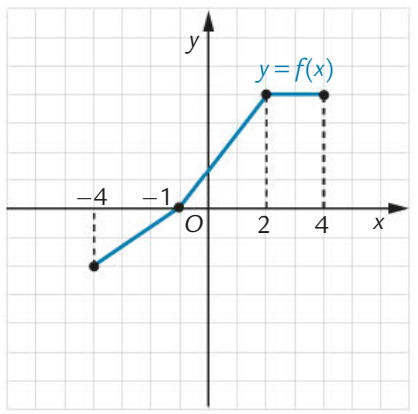
\includegraphics[width=0.35\textwidth]{images/funzione_trasformazione.png}
\end{wrapfigure}
In figura è tracciato il grafico della funzione $y = f(x)$. Deduci e rappresenta il grafico della funzione $y'=f(x-2)+1$
\vspace{60pt}
\end{minipage}
\begin{solution}
$f(x-2)$ trasla il grafico di $f$ di 2 unità verso \emph{destra}; il $+1$ lo trasla di 1 unità verso l'\emph{alto}. Complessivamente ogni punto $(x_0,y_0)$ del grafico di $f$ va in $(x_0+2,\ y_0+1)$: si ridisegna la stessa curva spostata di vettore $(2,1)$.
\end{solution}
\end{question}

%---------------------------------------------------------------------------------%

\begin{question}[ID=5.3, subtitle={Grafico e disequazione con $f(x)=|x+2|$ e $g(x)=2-\frac12|x|$}, tags={trasformazioni geometriche, valore assoluto}, difficulty=media]
Definite le seguenti funzioni:
\[ f(x) = |x+2| \qquad\qquad g(x) = 2 - \dfrac{1}{2}|x| \]
\begin{enumerate}
\item Rappresentare il grafico di $f(x)$ e $g(x)$;
\item Risolvere graficamente la disequazione $|x+2| < 2 - \dfrac{1}{2}|x|$.
\end{enumerate}
\begin{solution}
\begin{enumerate}
\item $f(x)=|x+2|$: V con vertice $(-2,0)$, rami di pendenza $\pm1$. $g(x)=2-\tfrac12|x|$: V capovolta con vertice $(0,2)$, rami di pendenza $\mp\tfrac12$.
\item La disequazione $f(x)<g(x)$ è soddisfatta dove la V di $f$ sta \emph{sotto} la $\Lambda$ di $g$. Si trovano le ascisse di intersezione studiando i casi del valore assoluto:
\begin{itemize}
\item $x<-2$: $-x-2<2+\tfrac{x}{2}\Rightarrow x>-\tfrac83$;
\item $-2\le x<0$: $x+2<2+\tfrac{x}{2}\Rightarrow x<0$ (sempre vero nell'intervallo);
\item $x\ge0$: $x+2<2-\tfrac{x}{2}\Rightarrow x<0$ (mai).
\end{itemize}
Unendo: $-\dfrac83<x<0$. (Agli estremi $x=-\tfrac83$ e $x=0$ i due grafici si toccano: $f=g$.)
\end{enumerate}
\end{solution}
\end{question}

%---------------------------------------------------------------------------------%

\begin{question}[ID=5.4, subtitle={Grafico e disequazione con $f(x)=|x-2|-1$ e $g(x)=2|x|-2$}, tags={trasformazioni geometriche, valore assoluto}, difficulty=media]
Definite le seguenti funzioni:
\[ f(x) = |x-2|-1 \qquad\qquad g(x) = 2|x|-2 \]
\begin{enumerate}
\item Rappresentare il grafico di $f(x)$ e $g(x)$;
\item Risolvere graficamente la disequazione $g(x) < f(x)$.
\end{enumerate}
\begin{solution}
\begin{enumerate}
\item $f(x)=|x-2|-1$: V con vertice $(2,-1)$, pendenze $\pm1$. $g(x)=2|x|-2$: V con vertice $(0,-2)$, rami più ripidi (pendenze $\pm2$).
\item $g(x)<f(x)\Leftrightarrow 2|x|-|x-2|<1$. Studiando i casi:
\begin{itemize}
\item $x<0$: $-2x-(2-x)=-x-2<1\Rightarrow x>-3$;
\item $0\le x<2$: $2x-(2-x)=3x-2<1\Rightarrow x<1$;
\item $x\ge2$: $2x-(x-2)=x+2<1\Rightarrow x<-1$ (mai).
\end{itemize}
Unendo: $-3<x<1$. (Agli estremi $x=-3$ e $x=1$ risulta $g=f$.)
\end{enumerate}
\end{solution}
\end{question}
